\documentclass{acm_proc_article-sp}
\usepackage{wrapfig}
\usepackage{tikz, alex, url, mu}
\usetikzlibrary{arrows,shapes,snakes,automata,backgrounds,petri}
\tikzset{>=stealth}

\title{Quilting for Distributed Machine Learning System}

\author{Mu Li \\ CMU CSD \and Jinliang Wei\\ CMU CSD}

\begin{document}
\maketitle

\begin{abstract}
In this paper we proposal QuiltDB, a distributed database optimized for network
topology.
\end{abstract}

\section{Introduction}

In distributed machine learning applications, data as well as computation are
partitioned among hundreds or  thousands of machines. Those
worker machines compute local results based on their own data. Global solutions
are then obtained via synchronization.

Machine synchronization, including data communication and waiting, is typically
the most expensive operation, because of limited network bandwidth and highly
variant machine performances. Recently, asynchronous communication is proposed
to hide the synchronization cost, however, those works assume the network has
uniform point-to-point bandwidth.

However, the real data datacenter network usually has specially topology. For
example, machines are grouped by ranks, and those ranks are then connected by
several layers of switchers. It thus forms a (multi-)tree like
topology. Machines within a rack has much larger bandwidth than crossing racks.

It is necessary to consider the network topology, because of the huge amount of
data communication volume and iterative nature of  machine learning
applications. In addition, if the communication forms a simple pattern, such as
a ring or a start, then it is much easier to improve the machine network
according this to pattern than improve the overall point-to-point bandwidth.

On this paper, we propose a database execute engine, QuiltDB, which mapping
machine learning applications into network topologies. Key features of this
system includes,

\begin{itemize*}
\item Allow use-defined network topology.
\item Model machine learning applications by the primal-dual decomposition.
\item A discrete streaming system.
\end{itemize*}



\section{Network Topologies}

On this section, we overview several common network topolgies.
\subsection{Grid}
\subsection{Star}

\section{Machine Learning Applications}

\subsection{Pagerank}
\subsection{Loss minimization}

\section{Implementation}
In this section, we discuss our system implementation along with techniques to 
minimize communication cost.

\subsection{Propagator-Receiver Pair}

Each physical node runs one QuiltDB process. The architecture of a single 
QuiltDB process is visualized in Fig~\ref{fig:prop-recv}.  The QuiltDB process
contains a set of application threads which execute application procedures and 
access the distributed paramters via the QuiltDB stub. 

The core of a QuiltDB stub is a paired propagator-receiver structure, which is 
referred to as \emph{logical node}. Namely the propagator-receiver pair consists
of a receiver, a propagator and a set of tables registered with this 
\emph{logical node}. The \emph{logical node} serves read and write accesses to 
key-value pairs, batches and aggregates operation logs for writes and propagate 
them to other QuiltDB processes, receives incoming operation logs and act upon 
received operation logs appropriately according to corresponding table 
configurations. One \emph{logical node} lets the QuiltDB process to participate 
in one update propagation path
A QuiltDB stub may contain multiple \emph{logical nodes} and 
there is no limit on the number of \emph{logical node}s. Howerver, our current 
implementation supports up to two \emph{logical nodes} as that suffices the 
needs of most applications.

A \emph{logical node} may have multiple tables registered with it. Since QuiltDB
requires value stored in one table to be of the same size, supporting multiple 
tables allows QuiltDB to support multiple types of values. The underlying data 
storage of table is a concurrent hash table.

When application threads read a key via GET(), the value is served directly from
the concurrent hash table. When application threads write a key via INC(), the 
operation is applied to the concurrent hash table and a operation log is 
appended to the propagator OpLog queue. The propagator thread reads the 
operation log from the queue. Instead of sending out the operation log 
immediately, the propagator batches operation logs and aggregate them (see
Section~\ref{sec:update-aggreg} for more details) in order to minimize 
communication overhead. Batched operation logs are grouped by table ID and are
sent out every $n$ micro-seconds, where $n$ is a user-configurable parameter.

A \emph{logical node} may have at most one \emph{logical node} as its downstream
receiver.

\begin{figure}[th!]
  \centering
  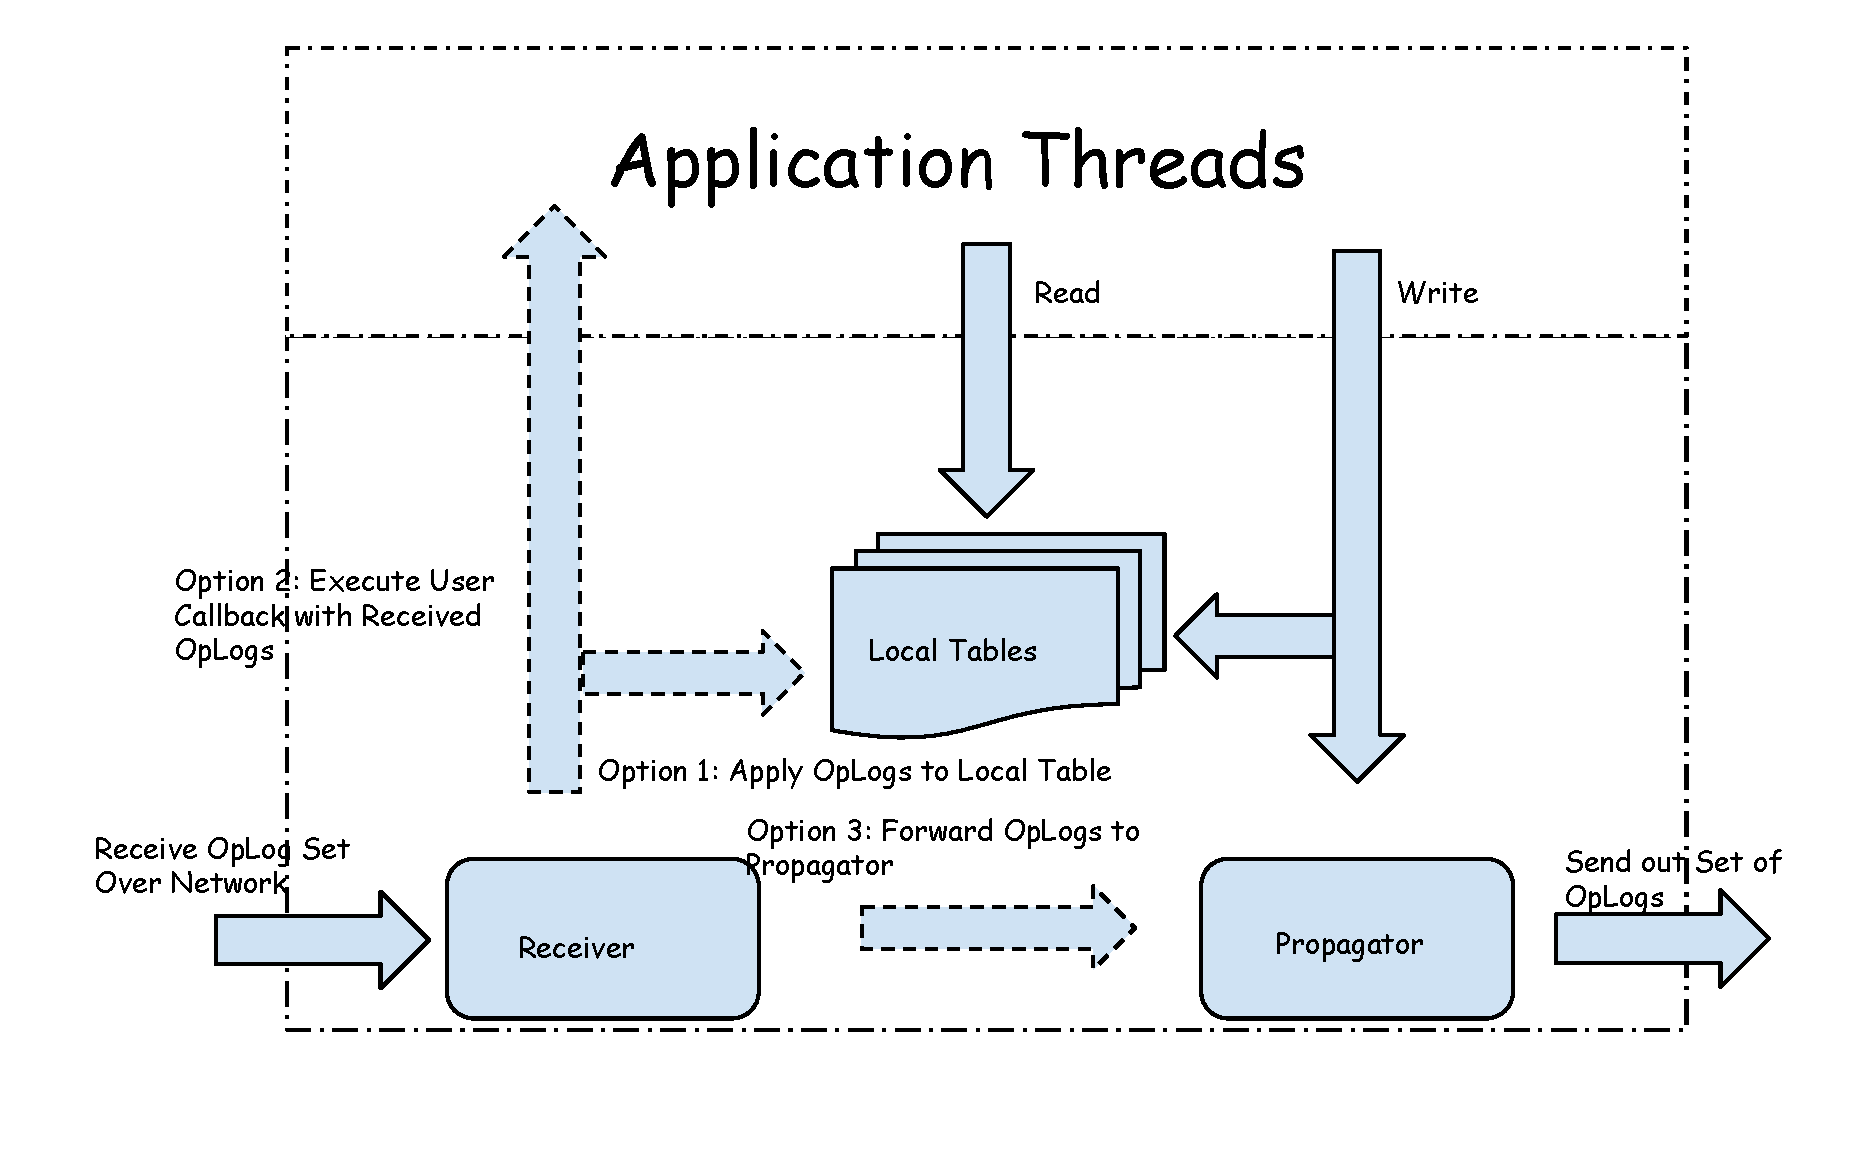
\includegraphics[width=.5\textwidth]{fig/propagator-receiver.pdf}
  \caption{Single Node Architecture}
  \label{fig:prop-recv}
\end{figure}

\subsection{Update Aggregration}
\label{sec:update-aggreg}

\subsection{Cyclic Path}

\section{Evaluation}

\appendix
\section{Project Overview}

We observe that for some machine learning algorithms and applications, we can
perform grid partitioning on data to minimize the amount of data to be
communicated. Moreover, for applications that tolerates long latency of updates,
we may organize worker nodes into a logic grid and restrict nodes to only
communicate with its neighbors to avoid the problem that some particular nodes
becomes the bottelneck of the entire system. Finally, by carefully reordering
data matrix in to diagonal block marix, we can futher reduce the
communication needed among nodes.

We realize that such quilting schem only applies to certain application
senarios. For example, the grid communication pattern has inevitably long
latency for update propagation, which requires the application to be able to
tolerate such long latency. In this project, we will investigate the above
techniques and aim at identifying application senarios where they may apply.

\subsection{Data Partition}
Different partitioning scheme requires different amount of data to be
communicated. For example, consider dual decomposition,
which iteratively executes two matrix multiplications:
\begin{align*}
w &= A \times u \\
u &= A^T \times w,
\end{align*}
where $A$ is a gigantic data matrix and $u$ and $w$ are two vectors.

Given a $n$-by-$m$ matrix $A$, we want to divide the matrix into $p$ machines
while minimizing the amount of data to be communicated in each iteration.

If we cut the matrix into $a$ rows and $b$ columns, then the minimal data
communication is

\begin{equation}
  r  am +  c bn
  \label{eq:total-traffic}
\end{equation}
where $r,c \in [0,1]$ are coefficient depending on the sparsity of the
matrix. They should be a function as $a$ and $b$, but now we consider it as a
constant to simply the calculation.

Note that $ab=p$, then (\ref{eq:total-traffic}) get minimize value when
$a = \rbr{ \frac{cn}{rm} }^{\frac{1}{2}}\sqrt{p}$. That is, if $cn \gg rm$, we
should choose partition scheme 1, if $rm \gg cn$, we should use scheme 2, while
if $rm \approx cn$, the even partition scheme 3 is a better choice.

\begin{figure}[th!]
  \centering
\begin{tikzpicture}[scale=.5]
  \draw [fill=set12!60](0,0) rectangle (4,1)
  rectangle (0,2) rectangle (4,3) rectangle (0,4);
  \draw[xshift=6cm, fill=set11!60] (0,0) rectangle (1,4) rectangle (2,0) rectangle (3,4)
  rectangle (4,0);
  \draw[xshift=12cm, fill=set13!60] (0,0) rectangle (2,2) rectangle (0,4);
  \draw[xshift=14cm, fill=set13!60] (0,0) rectangle (2,2) rectangle (0,4);
\end{tikzpicture}
  \caption{partition scheme 1 to 3: $a=4,b=1$, $a=1,b=4$, and $a=2,b=2$}
\end{figure}


\subsection{Data Communication}

\vskip 2ex

\begin{figure}[th!]
  \centering
  \begin{tikzpicture}[scale=.9]
    \tikzstyle{block} = [rectangle, draw, minimum size=1.6cm, text centered, rounded
    corners, minimum height=.8cm, font=\bf, text=white, thick]

    \foreach \i/\x in {0/0,1/2,2/4,3/8} {
      \node [block,fill=set12!80]  (s\i) at (\x cm, 2cm) {Server};
    }

    \foreach \i/\x in {0/0,1/2,2/4,3/8} {
      \node [block,fill=set13!80] (n\i) at (\x cm, 0cm) {Client};
    }

    \node at (6cm,2cm) {{\large $\cdots$}};
    \node at (6cm,0cm) {{\large $\cdots$}};
    \foreach \i in {0,1,2,3} {
      \foreach \j in {0,1,2,3} {
        \draw[<->, >=stealth,thick]  (n\i.north) -- (s\j.south);
      }
    }
  \end{tikzpicture}
  \caption{Parameter Server}
\end{figure}


As described, when used for sharing access to parameters, parameter server
can be easily overloaded and become the bottelneck of the system, especially
when the problem size and number of nodes scale up. Also, the free communication
pattern in the parameter server approach may easily congest the upper-tier links
of the tree network topology commonly seen in today's datacenter networks.

Instead of allowing nodes to freely communcate with each other, in our
framewrok, we propose a restricted communication paradigm where nodes form a
grid and each node only communicates with its logical neighbors in the grid, as
shown in Fig~\ref{fig:grid}. As each node only communicates with its neighbors,
such simple communication pattern effectively avoids the risk of loading a
single node.

%\begin{figure}[th!]
%\centering
%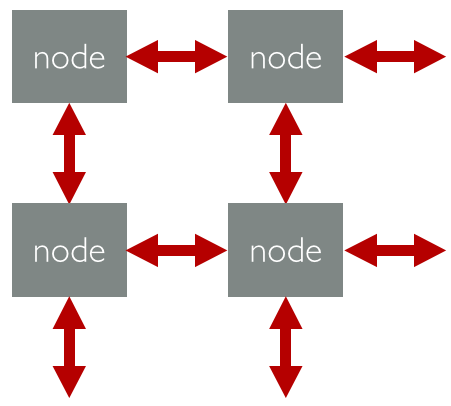
\includegraphics[width=0.35\textwidth]{grid.pdf}
%\caption{Grid communication pattern}
%\label{fig:grid}
%\end{figure}


\subsection{Data Processing}

Most large scale data are sparse and compressionable. Figure \ref{fig:block}
demonstrates an example that a sparse matrix can be reordered in rows and columns
to get a block form~\cite{Kang_beyond‘caveman}. Given a near diagonal block
matrix, it is better to maitain a whole block in a single machine, and that
machine will also be the ``master'' for the parameters, namely $u$ and $w$ in
our example, of this block, denoted by $u_b$ and $w_b$. Then only a small
portion of $u_b$ and $w_b$ will be shared outside this machine. The data
communication of this block of parameter, therefore, reduced.
\begin{figure}[th!]
  \centering
\begin{tikzpicture}[scale=.5]
  \draw[fill=set13!60] (0,0) rectangle (2,2) rectangle (4,4);
  \draw[] (4,0) rectangle (2,2) rectangle (0,4);
\end{tikzpicture}
  \caption{A block diagnal matrix}
\end{figure}


However, the methods proposed in \cite{Kang_beyond‘caveman} cannot be scaled to
very large datasets. We need to design more efficient data precessing method.

\begin{figure}[th!]
  \centering
  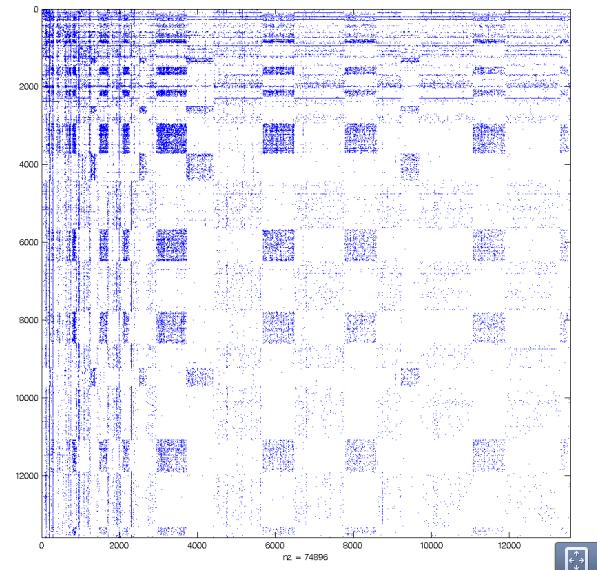
\includegraphics[width=.4\textwidth]{block}
  \caption{reordering of a real sparse matrix}
  \label{fig:block}
\end{figure}

\section{Experiments}

We shall implement one or a few distirbuted machine learning algorithms, such as
 linear regression, LDA topic modeling and deep neural network. The
implementation will be evaluated against real datasets and the evaluation will
be run on PDL's clusters.

\section{Agenda}

\begin{itemize*}
\item read some hpc grid-computing papers: 2 weeks
\item decide the communication patterns: 2 weeks
\item implementation: 2 weeks
\item evaluation: 2 weeks
\item writing final report: 1 week
\end{itemize*}

\appendix
\section{Acknowledgements}
The authors would like thank to Alex Smola, Dave Andersen (potentially more...)
for helpful discussion.

\bibliography{ref}
\bibliographystyle{abbrvnat}

\end{document}
